\documentclass[a4paper,11pt]{article}

\usepackage[utf8]{inputenc}
\usepackage[T1]{fontenc}
\usepackage[ngerman]{babel}
\usepackage[a4paper,margin=2.5cm]{geometry}
\usepackage{graphicx}
\usepackage{float}
\usepackage{hyperref}
\usepackage{enumitem}
\usepackage{parskip}
\usepackage{xcolor}

\hypersetup{
    colorlinks=true,
    linkcolor=blue,
    urlcolor=blue
}

\title{Buzzerino -- Aufbauanleitung}
\author{}
\date{}

\begin{document}

\maketitle

Diese Anleitung beschreibt den Aufbau des \textbf{Buzzerino}-Bausatzes Schritt für Schritt. Sie richtet sich an Studierende ohne oder mit nur wenig Löterfahrung. Ziel ist ein sauber aufgebautes und funktionsfähiges System.

\section*{Vorbereitung}

Bevor du beginnst, solltest du deinen Arbeitsplatz sinnvoll vorbereiten. Lege alle Bauteile übersichtlich bereit und prüfe, ob das notwendige Werkzeug vorhanden ist.

Benötigt werden:
\begin{itemize}
    \item Lötkolben
    \item Lötzinn
    \item Seitenschneider
    \item ggf. kleine Flachzange
    \item alle Bauteile des Bausatzes
\end{itemize}

\textbf{Hinweise zum Arbeiten:}
\begin{itemize}
    \item Arbeite konzentriert und ohne Zeitdruck.
    \item Der Lötkolben wird sehr heiß. Vermeide jeden Kontakt mit Spitze und frisch gelöteten Stellen.
    \item Löte möglichst sauber und mit wenig, aber ausreichend Lötzinn.
    \item Bei Bauteilen mit vielen Pins empfiehlt es sich fast immer, zunächst nur einen oder zwei Pins zu löten, die Ausrichtung zu prüfen und erst danach vollständig zu verlöten.
\end{itemize}

\section*{Stückliste}

\begin{figure}[H]
    \centering
    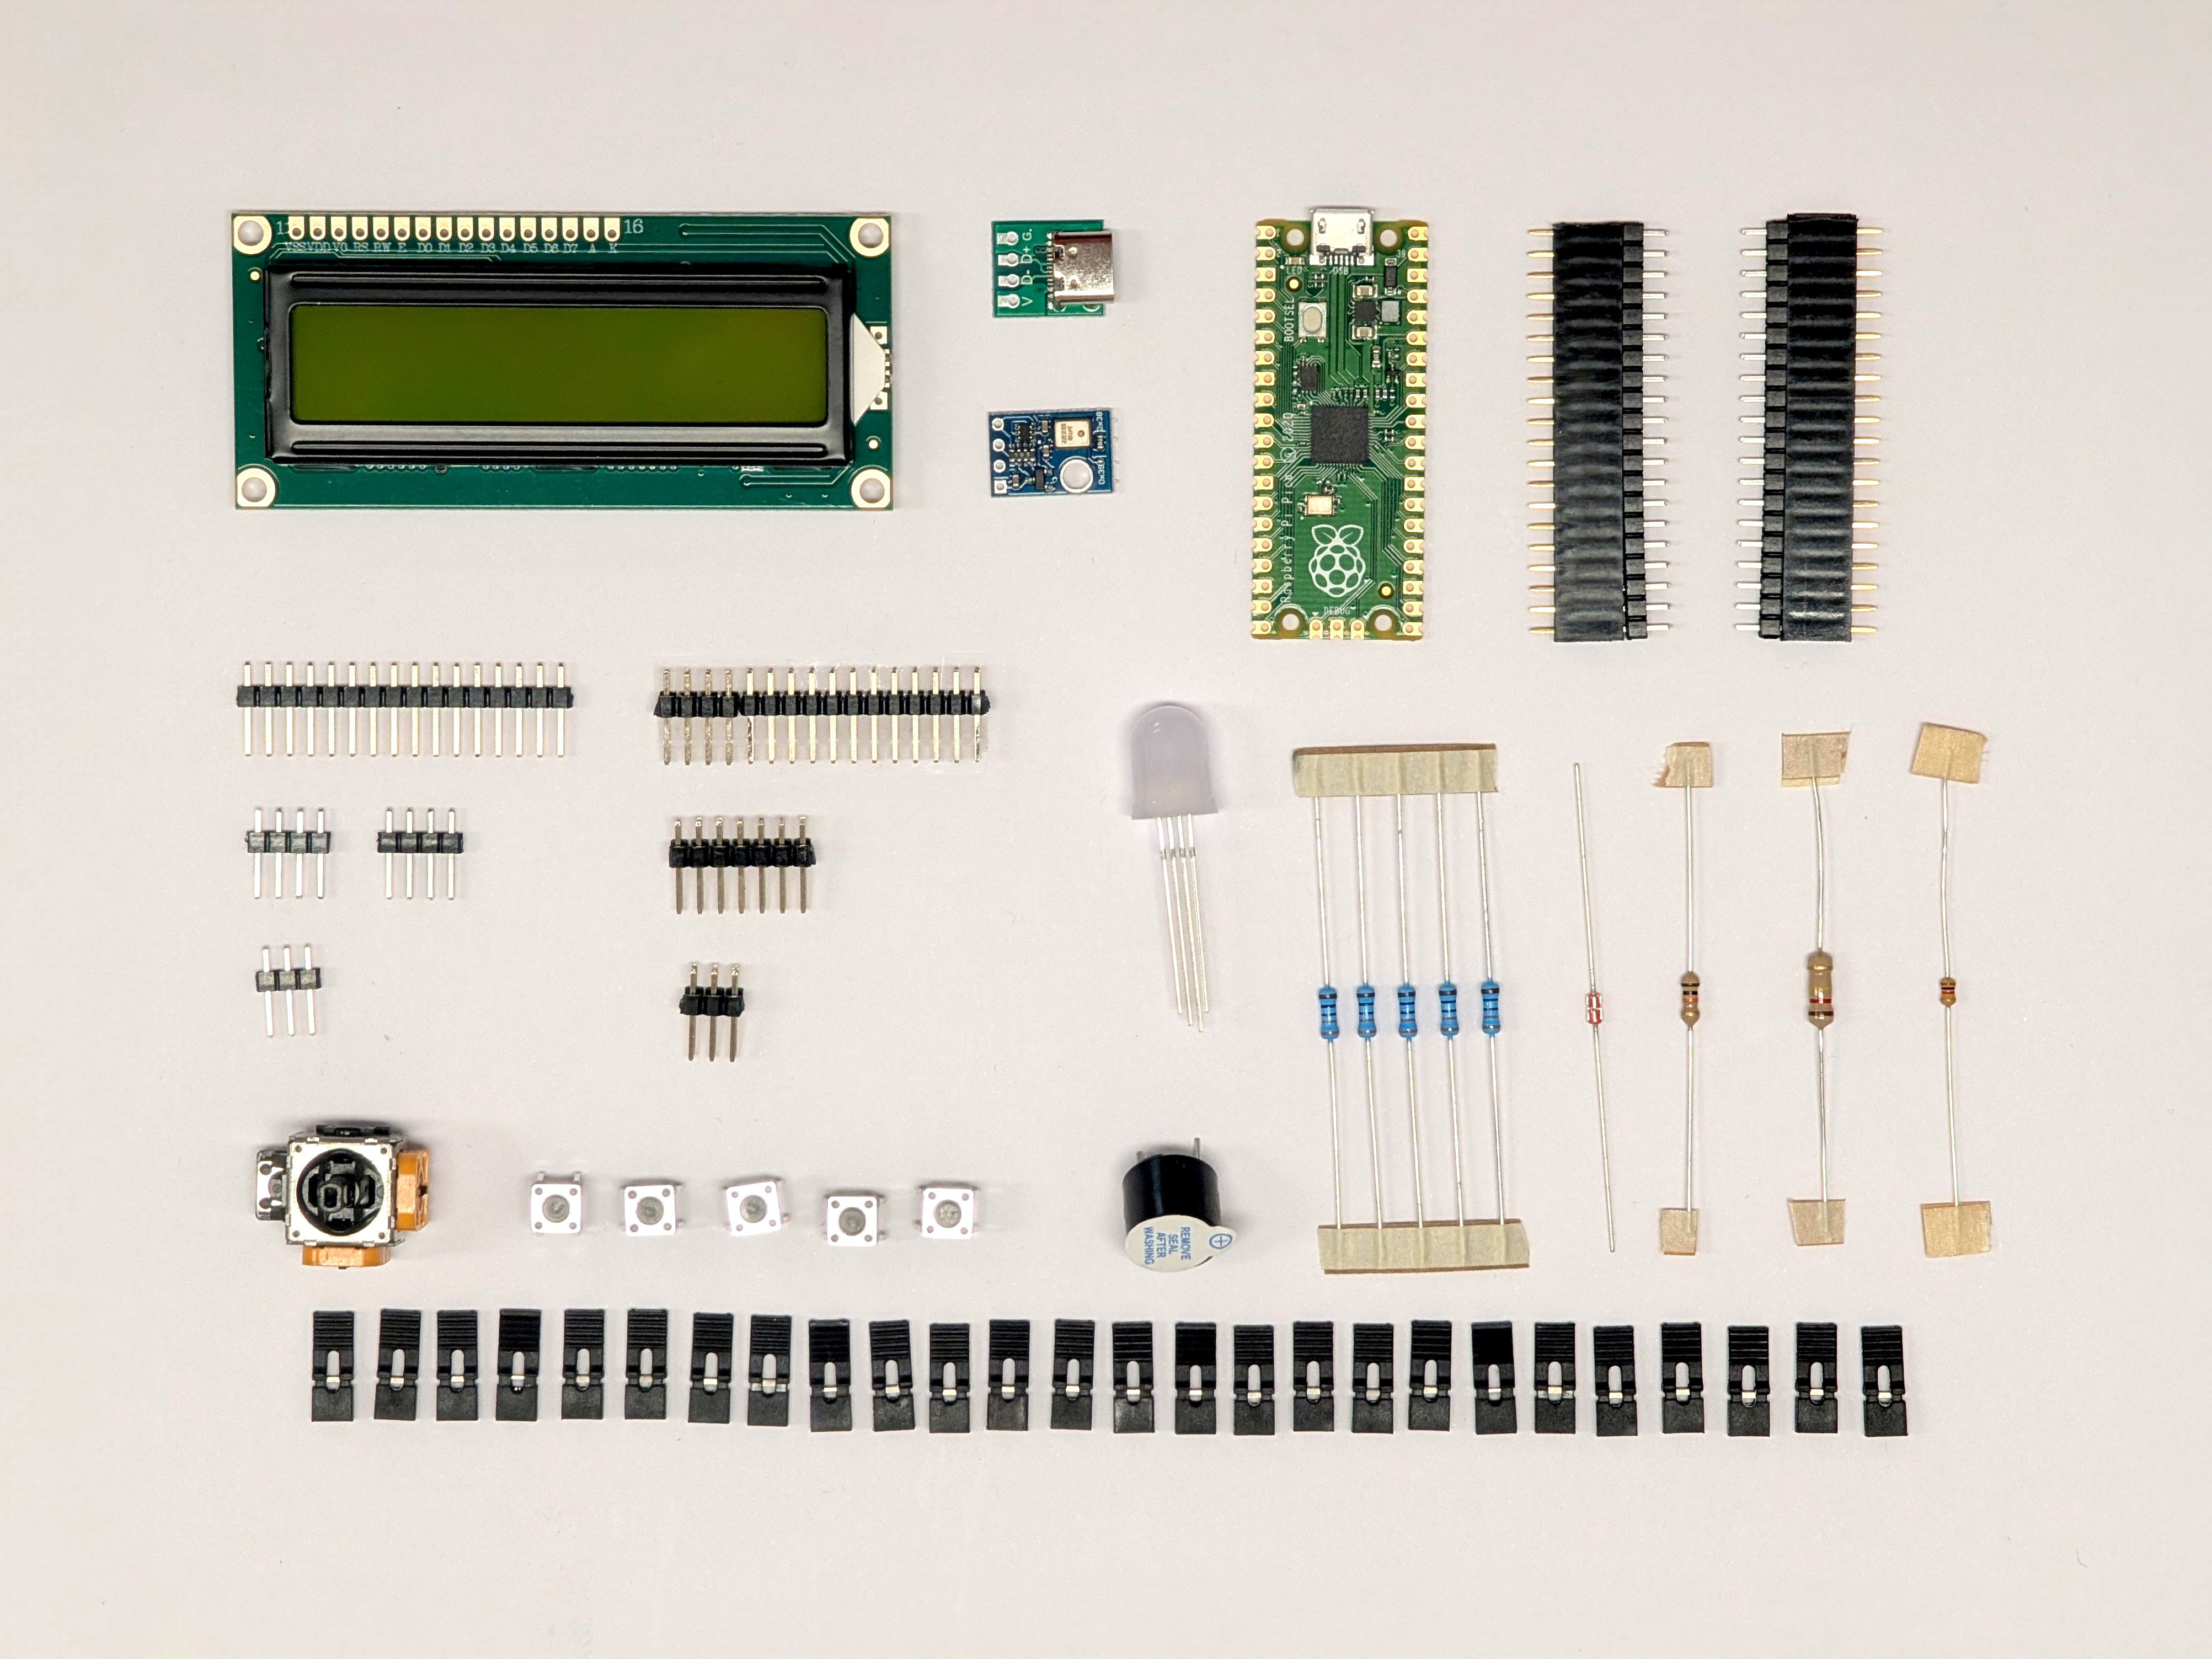
\includegraphics[width=0.8\textwidth]{images/overview_without_pcb.jpg}
\end{figure}

Vor dem Aufbau sollte kontrolliert werden, ob alle Komponenten vorhanden sind:

\begin{itemize}
    \item 1x Buzzerino-Platine
    \item 1x Raspberry Pi Pico
    \item 1x 1602A-LCD-Display
    \item 1x AHT10 Temperatur- und Luftfeuchtigkeitssensor
    \item 1x USB-C-Breakout-Board
    \item 1x 10\,mm RGB-LED
    \item 1x Buzzer
    \item 1x analoger Joystick
    \item 5x Taster
    \item 1x 100-k$\Omega$-NTC
    \item 5x 330-$\Omega$-Widerstände
    \item 1x 1-k$\Omega$-Widerstand
    \item 1x 10-k$\Omega$-Widerstand
    \item 1x 120-k$\Omega$-Widerstand
    \item 2x 1x20 Stift-/Buchsenleisten
    \item 1x 1x16 Stiftleiste
    \item 2x 1x4 Stiftleisten
    \item 1x 1x3 Stiftleiste
    \item 1x 2x16 Stiftleiste
    \item 1x 2x7 Stiftleiste
    \item 1x 2x3 Stiftleiste
    \item 26 Jumper
\end{itemize}

\section*{Grundprinzip beim Löten}

Für viele Schritte gilt dieselbe Vorgehensweise:
\begin{enumerate}
    \item Bauteil einsetzen
    \item zunächst nur einen Pin bzw. zwei gegenüberliegende Pins löten
    \item Ausrichtung kontrollieren
    \item gegebenenfalls korrigieren
    \item anschließend vollständig verlöten
\end{enumerate}

Dieses Vorgehen reduziert Fehler deutlich und erleichtert die Montage vor allem bei Steckleisten, Modulen und Bauteilen mit vielen Anschlüssen.

\section*{1. Raspberry Pi Pico vorbereiten}

Zunächst werden die beiden langen Stift-/Buchsenleisten mit dem Raspberry Pi Pico verlötet.

Wichtig ist dabei:
\begin{itemize}
    \item Die Leisten bestehen jeweils aus zwei zusammengesteckten Teilen.
    \item Diese sollten während des Lötens zusammengesteckt bleiben, damit die Pins sauber ausgerichtet sind.
    \item Die Seite mit dem schmaleren Kunststoffteil wird an den Raspberry Pi Pico gelötet.
\end{itemize}

\begin{figure}[H]
    \centering
    
\includegraphics[width=0.75\textwidth]{images/instruction_step_1.jpg}
\end{figure}

Vorgehen:
\begin{enumerate}
    \item Stiftleisten in Raspberry Pi Pico und Buzzerino-Platine einsetzen.
    \item Darauf achten, dass der Pico plan und parallel sitzt.
    \item Zunächst die vier Eckpins löten.
    \item Sitz und Ausrichtung kontrollieren.
    \item Den Pico wieder aus der Buzzerino-Platine entnehmen.
    \item Anschließend alle verbleibenden Pins vollständig verlöten.
\end{enumerate}

\begin{figure}[H]
    \centering
    
\includegraphics[width=0.75\textwidth]{images/instruction_step_2.jpg}
\end{figure}

\begin{figure}[H]
    \centering
    
\includegraphics[width=0.75\textwidth]{images/instruction_step_3.jpg}
\end{figure}

\begin{figure}[H]
    \centering
    
\includegraphics[width=0.75\textwidth]{images/instruction_step_4.jpg}
\end{figure}

\begin{figure}[H]
    \centering
    
\includegraphics[width=0.75\textwidth]{images/instruction_step_5.jpg}
\end{figure}

\begin{figure}[H]
    \centering
    
\includegraphics[width=0.75\textwidth]{images/instruction_step_6.jpg}
\end{figure}

\section*{2. USB-C-Breakout-Board vorbereiten}

Als Nächstes wird die 1x4-Stiftleiste an das USB-C-Breakout-Board gelötet.

\begin{figure}[H]
    \centering
    
\includegraphics[width=0.75\textwidth]{images/instruction_step_7.jpg}
\end{figure}

Vorgehen:
\begin{enumerate}
    \item Stiftleiste in das Breakout-Board einsetzen.
    \item Zunächst nur einen Pin löten.
    \item Ausrichtung prüfen; die Leiste sollte senkrecht zur Platine stehen.
    \item Falls nötig die erste Lötstelle erneut erwärmen und die Position korrigieren.
    \item Danach alle Pins vollständig löten.
\end{enumerate}

\begin{figure}[H]
    \centering
    
\includegraphics[width=0.75\textwidth]{images/instruction_step_8.jpg}
\end{figure}

\begin{figure}[H]
    \centering
    
\includegraphics[width=0.75\textwidth]{images/instruction_step_9.jpg}
\end{figure}

\begin{figure}[H]
    \centering
    
\includegraphics[width=0.75\textwidth]{images/instruction_step_10.jpg}
\end{figure}

\begin{figure}[H]
    \centering
    
\includegraphics[width=0.75\textwidth]{images/instruction_step_11.jpg}
\end{figure}

\section*{3. AHT10-Sensor vorbereiten}

Der AHT10-Sensor wird analog zum USB-C-Breakout-Board vorbereitet.

\begin{figure}[H]
    \centering
    
\includegraphics[width=0.75\textwidth]{images/instruction_step_12.jpg}
\end{figure}

Vorgehen:
\begin{enumerate}
    \item Stiftleiste einsetzen
    \item einen Pin löten
    \item Ausrichtung prüfen
    \item alle übrigen Pins löten
\end{enumerate}

\begin{figure}[H]
    \centering
    
\includegraphics[width=0.75\textwidth]{images/instruction_step_13.jpg}
\end{figure}

\section*{4. LCD-Display vorbereiten}

Das LCD-Display wird in derselben Weise vorbereitet.

\begin{figure}[H]
    \centering
    
\includegraphics[width=0.75\textwidth]{images/instruction_step_14.jpg}
\end{figure}

Vorgehen:
\begin{enumerate}
    \item Stiftleiste einsetzen
    \item einen Pin anlöten
    \item Ausrichtung kontrollieren
    \item anschließend vollständig verlöten
\end{enumerate}

\begin{figure}[H]
    \centering
    
\includegraphics[width=0.75\textwidth]{images/instruction_step_15.jpg}
\end{figure}

\begin{figure}[H]
    \centering
    
\includegraphics[width=0.75\textwidth]{images/instruction_step_16.jpg}
\end{figure}

\section*{5. Widerstände einbauen}

Die Widerstände werden direkt auf der Buzzerino-Platine montiert. Vor dem Einsetzen müssen die Anschlussdrähte passend gebogen werden.

Allgemeines Vorgehen:
\begin{enumerate}
    \item Anschlussdrähte U-förmig biegen
    \item Bauteil einsetzen
    \item Drähte auf der Rückseite leicht spreizen, damit das Bauteil nicht herausfällt
    \item zunächst einen Anschluss löten
    \item Sitz kontrollieren
    \item zweiten Anschluss löten
    \item Drahtenden bündig kürzen
\end{enumerate}

\subsection*{5.1 NTC-Widerstand}

Der 100-k$\Omega$-NTC ist an seinem kleinen Glasgehäuse ohne Farbringe zu erkennen. Er wird an der Position \textbf{TH\_NTC} eingesetzt.

Wichtig:
\begin{itemize}
    \item Die bedruckte Seite der Platine ist die Vorderseite.
    \item In der linken unteren Ecke sollte das DIGITEC-Logo sichtbar sein.
\end{itemize}

\begin{figure}[H]
    \centering
    
\includegraphics[width=0.75\textwidth]{images/instruction_step_17.jpg}
\end{figure}

\begin{figure}[H]
    \centering
    
\includegraphics[width=0.75\textwidth]{images/instruction_step_18.jpg}
\end{figure}

\begin{figure}[H]
    \centering
    
\includegraphics[width=0.75\textwidth]{images/instruction_step_19.jpg}
\end{figure}

\begin{figure}[H]
    \centering
    
\includegraphics[width=0.75\textwidth]{images/instruction_step_20.jpg}
\end{figure}

\begin{figure}[H]
    \centering
    
\includegraphics[width=0.75\textwidth]{images/instruction_step_21.jpg}
\end{figure}

\begin{figure}[H]
    \centering
    
\includegraphics[width=0.75\textwidth]{images/instruction_step_22.jpg}
\end{figure}

\begin{figure}[H]
    \centering
    
\includegraphics[width=0.75\textwidth]{images/instruction_step_23.jpg}
\end{figure}

\begin{figure}[H]
    \centering
    
\includegraphics[width=0.75\textwidth]{images/instruction_step_24.jpg}
\end{figure}

\begin{figure}[H]
    \centering
    
\includegraphics[width=0.75\textwidth]{images/instruction_step_25.jpg}
\end{figure}

\begin{figure}[H]
    \centering
    
\includegraphics[width=0.75\textwidth]{images/instruction_step_26.jpg}
\end{figure}

\subsection*{5.2 1-k$\Omega$-Widerstand}

Farbcodierung:
\begin{itemize}
    \item Braun
    \item Schwarz
    \item Rot
    \item Gold
\end{itemize}

\begin{figure}[H]
    \centering
    
\includegraphics[width=0.75\textwidth]{images/instruction_step_27.jpg}
\end{figure}

\begin{figure}[H]
    \centering
    
\includegraphics[width=0.75\textwidth]{images/instruction_step_28.jpg}
\end{figure}

\begin{figure}[H]
    \centering
    
\includegraphics[width=0.75\textwidth]{images/instruction_step_29.jpg}
\end{figure}

\subsection*{5.3 10-k$\Omega$-Widerstand}

Farbcodierung:
\begin{itemize}
    \item Braun
    \item Schwarz
    \item Orange
    \item Gold
\end{itemize}

\begin{figure}[H]
    \centering
    
\includegraphics[width=0.75\textwidth]{images/instruction_step_30.jpg}
\end{figure}

\begin{figure}[H]
    \centering
    
\includegraphics[width=0.75\textwidth]{images/instruction_step_31.jpg}
\end{figure}

\begin{figure}[H]
    \centering
    
\includegraphics[width=0.75\textwidth]{images/instruction_step_32.jpg}
\end{figure}

\subsection*{5.4 330-$\Omega$-Widerstände}

Farbcodierung:
\begin{itemize}
    \item Orange
    \item Orange
    \item Schwarz
    \item Schwarz
    \item Braun
\end{itemize}

Von diesen Widerständen werden fünf Stück eingebaut.

\begin{figure}[H]
    \centering
    
\includegraphics[width=0.75\textwidth]{images/instruction_step_33.jpg}
\end{figure}

\begin{figure}[H]
    \centering
    
\includegraphics[width=0.75\textwidth]{images/instruction_step_34.jpg}
\end{figure}

\begin{figure}[H]
    \centering
    
\includegraphics[width=0.75\textwidth]{images/instruction_step_35.jpg}
\end{figure}

\begin{figure}[H]
    \centering
    
\includegraphics[width=0.75\textwidth]{images/instruction_step_36.jpg}
\end{figure}

\subsection*{5.5 120-k$\Omega$-Widerstand}

Farbcodierung:
\begin{itemize}
    \item Braun
    \item Rot
    \item Gelb
    \item Gold
\end{itemize}

\begin{figure}[H]
    \centering
    
\includegraphics[width=0.75\textwidth]{images/instruction_step_37.jpg}
\end{figure}

\begin{figure}[H]
    \centering
    
\includegraphics[width=0.75\textwidth]{images/instruction_step_38.jpg}
\end{figure}

\begin{figure}[H]
    \centering
    
\includegraphics[width=0.75\textwidth]{images/instruction_step_39.jpg}
\end{figure}

\section*{6. Taster einbauen}

Als Nächstes werden die fünf Taster montiert.

\begin{itemize}
    \item ein Reset-Taster
    \item vier Taster für das D-Pad
\end{itemize}

Wichtig ist, dass die Taster vollständig eingesetzt sind und plan auf der Platine aufliegen, bevor sie verlötet werden.

\begin{figure}[H]
    \centering
    
\includegraphics[width=0.75\textwidth]{images/instruction_step_40.jpg}
\end{figure}

\begin{figure}[H]
    \centering
    
\includegraphics[width=0.75\textwidth]{images/instruction_step_41.jpg}
\end{figure}

\begin{figure}[H]
    \centering
    
\includegraphics[width=0.75\textwidth]{images/instruction_step_42.jpg}
\end{figure}

\begin{figure}[H]
    \centering
    
\includegraphics[width=0.75\textwidth]{images/instruction_step_43.jpg}
\end{figure}

\section*{7. Stiftleisten auf die Hauptplatine löten}

Nun werden mehrere Stiftleisten direkt auf die Buzzerino-Platine gelötet.

\textbf{Wichtiger Hinweis:}  
Die \textbf{kurze Seite} der Pins muss durch die Platine gesteckt werden. Das ist eine häufige Fehlerquelle.

Einzubauen sind:
\begin{itemize}
    \item 2x7-Stiftleiste
    \item 2x3-Stiftleiste
    \item 2x16-Stiftleiste
    \item 1x3-Stiftleiste
\end{itemize}

Empfohlenes Vorgehen:
\begin{enumerate}
    \item Leiste einsetzen
    \item zunächst einen Pin löten
    \item Sitz und Rechtwinkligkeit kontrollieren
    \item gegebenenfalls korrigieren
    \item restliche Pins verlöten
\end{enumerate}

\begin{figure}[H]
    \centering
    
\includegraphics[width=0.75\textwidth]{images/instruction_step_44.jpg}
\end{figure}

\begin{figure}[H]
    \centering
    
\includegraphics[width=0.75\textwidth]{images/instruction_step_45.jpg}
\end{figure}

\begin{figure}[H]
    \centering
    
\includegraphics[width=0.75\textwidth]{images/instruction_step_46.jpg}
\end{figure}

\begin{figure}[H]
    \centering
    
\includegraphics[width=0.75\textwidth]{images/instruction_step_47.jpg}
\end{figure}

\begin{figure}[H]
    \centering
    
\includegraphics[width=0.75\textwidth]{images/instruction_step_48.jpg}
\end{figure}

\begin{figure}[H]
    \centering
    
\includegraphics[width=0.75\textwidth]{images/instruction_step_49.jpg}
\end{figure}

\begin{figure}[H]
    \centering
    
\includegraphics[width=0.75\textwidth]{images/instruction_step_50.jpg}
\end{figure}

\begin{figure}[H]
    \centering
    
\includegraphics[width=0.75\textwidth]{images/instruction_step_51.jpg}
\end{figure}

\begin{figure}[H]
    \centering
    
\includegraphics[width=0.75\textwidth]{images/instruction_step_52.jpg}
\end{figure}

\section*{8. USB-C-Breakout-Board einbauen}

Das vorbereitete USB-C-Breakout-Board wird an der rechten Seite der Hauptplatine montiert. Der USB-Anschluss muss nach außen zeigen und vollständig sichtbar sein.

Vorgehen:
\begin{enumerate}
    \item Modul einsetzen
    \item einen Pin löten
    \item Ausrichtung kontrollieren; das Modul sollte parallel zur Hauptplatine stehen
    \item anschließend vollständig verlöten
\end{enumerate}

\textbf{Hinweis:} Die Pins dieses Moduls sind relativ hart. Zum Kürzen sollte ein größerer Drahtschneider verwendet werden.

\begin{figure}[H]
    \centering
    
\includegraphics[width=0.75\textwidth]{images/instruction_step_53.jpg}
\end{figure}

\begin{figure}[H]
    \centering
    
\includegraphics[width=0.75\textwidth]{images/instruction_step_54.jpg}
\end{figure}

\begin{figure}[H]
    \centering
    
\includegraphics[width=0.75\textwidth]{images/instruction_step_55.jpg}
\end{figure}

\begin{figure}[H]
    \centering
    
\includegraphics[width=0.75\textwidth]{images/instruction_step_56.jpg}
\end{figure}

\section*{9. AHT10-Sensor einbauen}

Der AHT10-Sensor wird auf der linken Seite der Hauptplatine montiert. Die Bauteile auf dem Sensormodul sollten sichtbar nach außen zeigen.

Vorgehen:
\begin{enumerate}
    \item Sensor einsetzen
    \item einen Pin löten
    \item Ausrichtung kontrollieren
    \item vollständig verlöten
\end{enumerate}

Auch hier gilt: zum Kürzen der Pins besser einen größeren Drahtschneider verwenden.

\begin{figure}[H]
    \centering
    
\includegraphics[width=0.75\textwidth]{images/instruction_step_57.jpg}
\end{figure}

\begin{figure}[H]
    \centering
    
\includegraphics[width=0.75\textwidth]{images/instruction_step_58.jpg}
\end{figure}

\section*{10. Buzzer einbauen}

Der Buzzer ist ein \textbf{polarisiertes} Bauteil und muss korrekt ausgerichtet werden.

Beachte:
\begin{itemize}
    \item Auf der Platine ist die positive Seite mit \textbf{+} markiert.
    \item Auf dem Buzzer ist die positive Seite ebenfalls markiert.
    \item Der längere Anschlussdraht ist der Pluspol.
\end{itemize}

Beim Einsetzen müssen diese Merkmale übereinstimmen.

\begin{figure}[H]
    \centering
    
\includegraphics[width=0.75\textwidth]{images/instruction_step_59.jpg}
\end{figure}

\begin{figure}[H]
    \centering
    
\includegraphics[width=0.75\textwidth]{images/instruction_step_60.jpg}
\end{figure}

\section*{11. LCD-Display einbauen}

Das vorbereitete LCD-Display wird analog zu den anderen Modulen montiert.

Vorgehen:
\begin{enumerate}
    \item Display einsetzen
    \item einen Pin löten
    \item Sitz und Ausrichtung kontrollieren
    \item vollständig verlöten
\end{enumerate}

Zum Kürzen der Pins sollte ebenfalls ein größerer Drahtschneider verwendet werden.

\begin{figure}[H]
    \centering
    
\includegraphics[width=0.75\textwidth]{images/instruction_step_61.jpg}
\end{figure}

\begin{figure}[H]
    \centering
    
\includegraphics[width=0.75\textwidth]{images/instruction_step_62.jpg}
\end{figure}

\begin{figure}[H]
    \centering
    
\includegraphics[width=0.75\textwidth]{images/instruction_step_63.jpg}
\end{figure}

\begin{figure}[H]
    \centering
    
\includegraphics[width=0.75\textwidth]{images/instruction_step_64.jpg}
\end{figure}

\section*{12. RGB-LED einbauen}

Auch die RGB-LED ist polarisiert und muss korrekt eingesetzt werden.

Wichtig:
\begin{itemize}
    \item Das längste Bein ist hier der Minuspol.
    \item Auf der Platine ist der Minuspol durch ein quadratisches Pad gekennzeichnet.
\end{itemize}

Nach dem Löten und Kürzen der Anschlüsse kann die Lötstelle optisch unregelmäßig aussehen. In diesem Fall kann sie vorsichtig nacherwärmt werden. Dabei ist unbedingt darauf zu achten, dass keine Lötbrücken zwischen benachbarten Pins entstehen.

\begin{figure}[H]
    \centering
    
\includegraphics[width=0.75\textwidth]{images/instruction_step_65.jpg}
\end{figure}

\begin{figure}[H]
    \centering
    
\includegraphics[width=0.75\textwidth]{images/instruction_step_66.jpg}
\end{figure}

\begin{figure}[H]
    \centering
    
\includegraphics[width=0.75\textwidth]{images/instruction_step_67.jpg}
\end{figure}

\begin{figure}[H]
    \centering
    
\includegraphics[width=0.75\textwidth]{images/instruction_step_68.jpg}
\end{figure}

\begin{figure}[H]
    \centering
    
\includegraphics[width=0.75\textwidth]{images/instruction_step_70.jpg}
\end{figure}

\begin{figure}[H]
    \centering
    
\includegraphics[width=0.75\textwidth]{images/instruction_step_71.jpg}
\end{figure}

\section*{13. Raspberry Pi Pico einbauen}

Jetzt wird der vorbereitete Raspberry Pi Pico auf die Hauptplatine gesetzt.

Empfohlenes Vorgehen:
\begin{enumerate}
    \item Pico einsetzen
    \item zunächst zwei gegenüberliegende Pins löten
    \item Ausrichtung kontrollieren
    \item danach alle übrigen Pins löten
\end{enumerate}

\begin{figure}[H]
    \centering
    
\includegraphics[width=0.75\textwidth]{images/instruction_step_72.jpg}
\end{figure}

\begin{figure}[H]
    \centering
    
\includegraphics[width=0.75\textwidth]{images/instruction_step_73.jpg}
\end{figure}

\begin{figure}[H]
    \centering
    
\includegraphics[width=0.75\textwidth]{images/instruction_step_74.jpg}
\end{figure}

\section*{14. Joystick einbauen}

Der Joystick ist das letzte Bauteil und wegen seiner vielen Anschlüsse mechanisch etwas anspruchsvoller.

Vorgehen:
\begin{enumerate}
    \item Bauteil vorsichtig ansetzen
    \item zunächst die Tasterpins und danach die übrigen Pins in Position bringen
    \item das Bauteil vollständig einsetzen
    \item anschließend alle Pins verlöten
\end{enumerate}

Hier ist etwas Geduld hilfreich. Nicht mit Gewalt arbeiten; stattdessen das Bauteil langsam ausrichten.

\begin{figure}[H]
    \centering
    
\includegraphics[width=0.75\textwidth]{images/instruction_step_75.jpg}
\end{figure}

\begin{figure}[H]
    \centering
    
\includegraphics[width=0.75\textwidth]{images/instruction_step_76.jpg}
\end{figure}

\begin{figure}[H]
    \centering
    
\includegraphics[width=0.75\textwidth]{images/instruction_step_77.jpg}
\end{figure}

\begin{figure}[H]
    \centering
    
\includegraphics[width=0.75\textwidth]{images/instruction_step_78.jpg}
\end{figure}

\begin{figure}[H]
    \centering
    
\includegraphics[width=0.75\textwidth]{images/instruction_step_79.jpg}
\end{figure}

\section*{15. Jumper einsetzen}

Vor dem Testen der Platine müssen alle \textbf{26 Jumper} eingesetzt werden.

\begin{figure}[H]
    \centering
    
\includegraphics[width=0.75\textwidth]{images/instruction_step_80.jpg}
\end{figure}

Erst danach ist das System vollständig aufgebaut.

\section*{Abschluss}

Wenn alle Bauteile korrekt montiert und alle Jumper gesetzt sind, ist der Hardware-Aufbau abgeschlossen.

\textbf{Empfehlung vor dem ersten Einschalten:}
\begin{itemize}
    \item Sichtprüfung aller Lötstellen
    \item Kontrolle auf vergessene oder vertauschte Bauteile
    \item Kontrolle auf Lötbrücken, insbesondere bei eng beieinanderliegenden Pins
    \item Kontrolle der Polung bei Buzzer und RGB-LED
\end{itemize}

\section*{Programm aufspielen}

Falls auf dem Raspberry Pi Pico noch keine passende Firmware vorhanden ist, kann z.\,B. die Datei \texttt{self\_test.uf2} aufgespielt werden.

Vorgehen:
\begin{enumerate}
    \item BOOTSEL-Taste auf dem Raspberry Pi Pico gedrückt halten
    \item Pico per USB mit dem Rechner verbinden
    \item warten, bis das Laufwerk \textbf{RPI-RP2} erscheint
    \item \texttt{.uf2}-Datei auf dieses Laufwerk kopieren
    \item der Pico startet danach automatisch neu
\end{enumerate}

\section*{Praktische Hinweise}

\begin{itemize}
    \item Kurze, saubere Lötzeiten sind besser als langes Erhitzen.
    \item Bei Unsicherheit zunächst nur einen Pin löten und die Lage prüfen.
    \item Drahtenden immer erst nach erfolgreicher Positionierung kürzen.
    \item Wenn etwas nicht passt, nicht mit Kraft arbeiten, sondern die Ausrichtung erneut prüfen.
\end{itemize}

\end{document}